\documentclass[nouppercase]{ifmbe}
\usepackage{amsmath}

\title{Anomaly Detection Using Autoencoders for Movement Prediction}

\affiliation{Universidade de Brasília/Engenharia Biomédica, Brasília, Brasil }{FIRSTAFF}
\affiliation{Medical Biophysic Center, Santiago de Cuba, Cuba }{SECONDAFF}

\author{L.J.L. Barbosa}{FIRSTAFF}
\author{A.L. Delis}{SECONDAFF}
\author{P.V.P Cotta}{FIRSTAFF}
\author{V.O. Silva}{FIRSTAFF}
\author{M.D.C. Araujo}{FIRSTAFF}
\author{A. Rocha}{FIRSTAFF}

\begin{document}

\maketitle

\begin{abstract}

The smaller the time window, the faster the response of a prosthesis to the user's movement. However, very small windows have very little information, which makes it difficult to classify the sEMG signal. This article presents the use of autoencoders for the detection of motion in real time processing. For this purpose, a time window of .01s window (i.e., ten samplesper window). Through the difference between the number of peaks and the distance between them in the resulting latent space, it was possible to classify the moment when the patient starts to move. Through the use of autoencoder as an anomaly detector, it was possible to classify the beginning of the user's movement, thus managing to improve the classification in real time.

\end{abstract}

\begin{keywords}
EMG, Variational Autoencoder, .
\end{keywords}

\section{Introduction}

As we decrease the time frame of our analysis, the classification of the moment when the individual starts to move becomes very difficult, because of the amount of information decrease. Actually, in the classification of the EMG signal, it is more difficult to differentiate the signal patterns. So, the best way to classify it becomes the use of a priori information. The differentiation of the state of rest and movement becomes fundamental for the classification of movements, since rest is the class that most appears, it is also the one that has the highest entropy.

In this article, an anomaly detection method for the detection of movement was studied. Considering the normal state of rest, any disturbance in this state was treated as an anomaly. For this detection, an autoencoder was used.

An autoencoder is a neural network that is trained to attempt to copy its input to its output. While copying the input to the output may be useless, a high-dimensional data can be converted to low-dimensional codes by training a multilayer neural network with a small central layer to reconstruct high-dimensional input vectors. Using the inner layer, also called latent space, we have a signal with a reduced size, more easily classified.

The Variational Autoencoder (VAE) is a kind of autoencoder with a generative model that estimates the Probability Density Function (PDF) of training data. By training the model to recognize the sEMG signal it will assign a high probability value to a motion class, while the noise will receive a low probability value\cite{Welling}.

\subsection{Anomaly Detection}
The use of autoencoder for anomaly detection is already common in the area of artificial intelligence. Zong et al.~\cite{Zong2018} utilizes a deep autoencoder to generate a low-dimensional representation and reconstruction error for each input data point, which is further fed into a Gaussian Mixture Model (GMM) for anomaly detection. While Aytekin et al.~\cite{Aytekin2018} shows that an l2 normalization constraint improve the autoencoder representation. In this study, because it is highly specialized in separating classes in their latent space, a variational autoencoder was used to detect the beginning of the movement, which is otherwise confused with the resting state. This means that, although the VAE has a longer training time than a normal autoencoder, its final model will be shorter than that of another autoencoder for the same classification accuracy.

With the use of the autoencoder it was possible to decrease one of the dataset classes, the rest, which facilitated the posterior classification. Another advantage was the improvement in the response time of the classifier system to detect the beginning of the user's movement, which is extremely important for real-time processing, especially with such a small time window.

This paper is organized as follows: Section II shows a detailed explanation of the algorithms used. The results are listed in Section III, which also presents a detailed analysis of the experiment. Finally, there is a conclusion, where the results are summarized.

\section{Methodology}

Figure \ref{fig_flowchart} represent the flowchart of the anomaly detection. Through the analysis of the number of peaks, and the distance between them, it is possible to determine the beginning of the movement by the patient. A SVM was used for better generalization.

\begin{figure}[h]
\centering
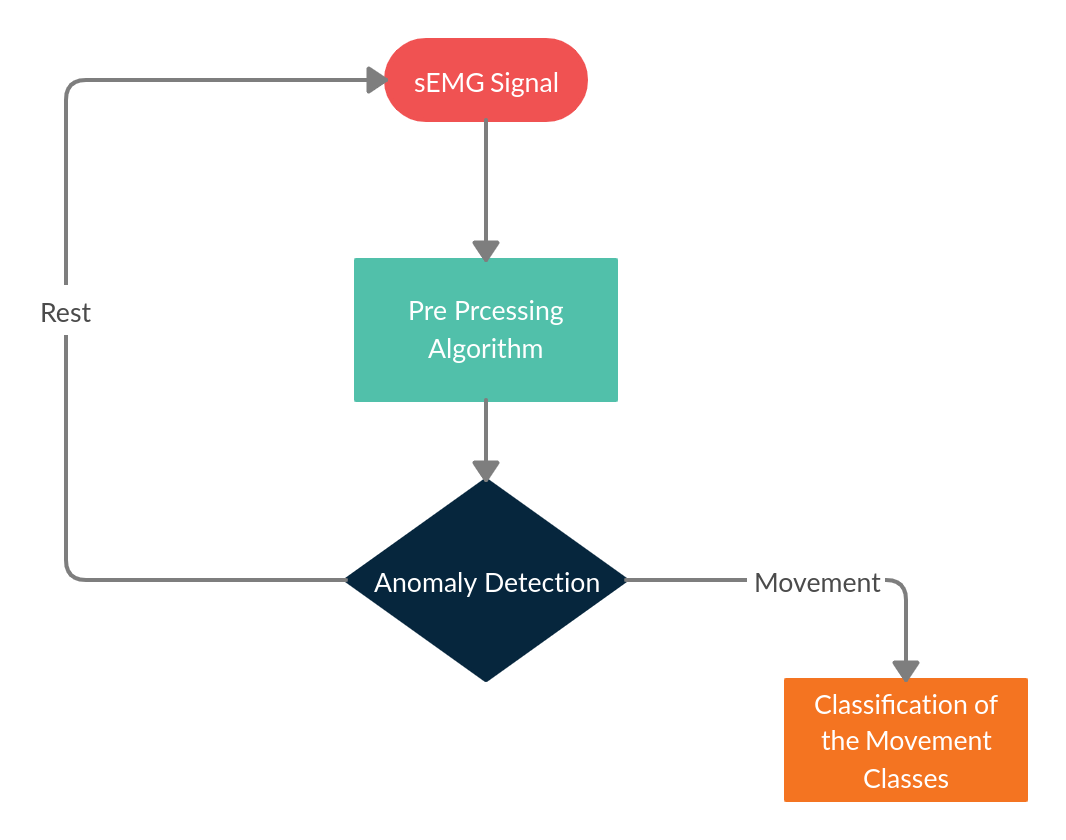
\includegraphics[width=.8\linewidth]{figuras/anomaly_detection.png}
\caption{Flowchart for the anomaly detection. Through the analysis of the number of peaks,  and the distance between them, extracted in the latent space by the VAE in the Anomaly Detection Block, it is possible to determine the beginning of the movement by the patient.} \label{fig_flowchart}
\end{figure}

\subsection{The VAE Model}

The VAE model can sample examples of the PDF learned, thus generating new examples similar to the original data set. But it is important to emphasize that VAE is not a way of training generative models, but rather that the generative model is a component of VAE, generally being a deeply latent Gaussian model\cite{Rezende2014}.

In the figure \ref{fig2} are the steps to summarize the operation of a VAE. On the left side we have the model definition:

\begin{enumerate}
    \item  Let $q(z|x)$ be defined as how the signal is encoded into a distribution over the latent space;
    \item  Let z be A latent vector sampled from $ q(z|x)$, $z$ will contain the information describing $x$. The decode of it is represented as $p(z|x)$;
    \item  $z$ is decoded as a signal.
\end{enumerate}

On the right side we have the loss:

\begin{enumerate}
    \item Reconstruction error: the difference between the output and the input.
    \item $p(z|x)$ should be similar to the prior (multivariate standard Gaussian).
\end{enumerate}

The VAE generating coefficient appears by directly sampling the latent vector from the prior distribution and decoding it into a noisy representation of $x$\cite{Welling}.

\begin{figure}
	\begin{center}
	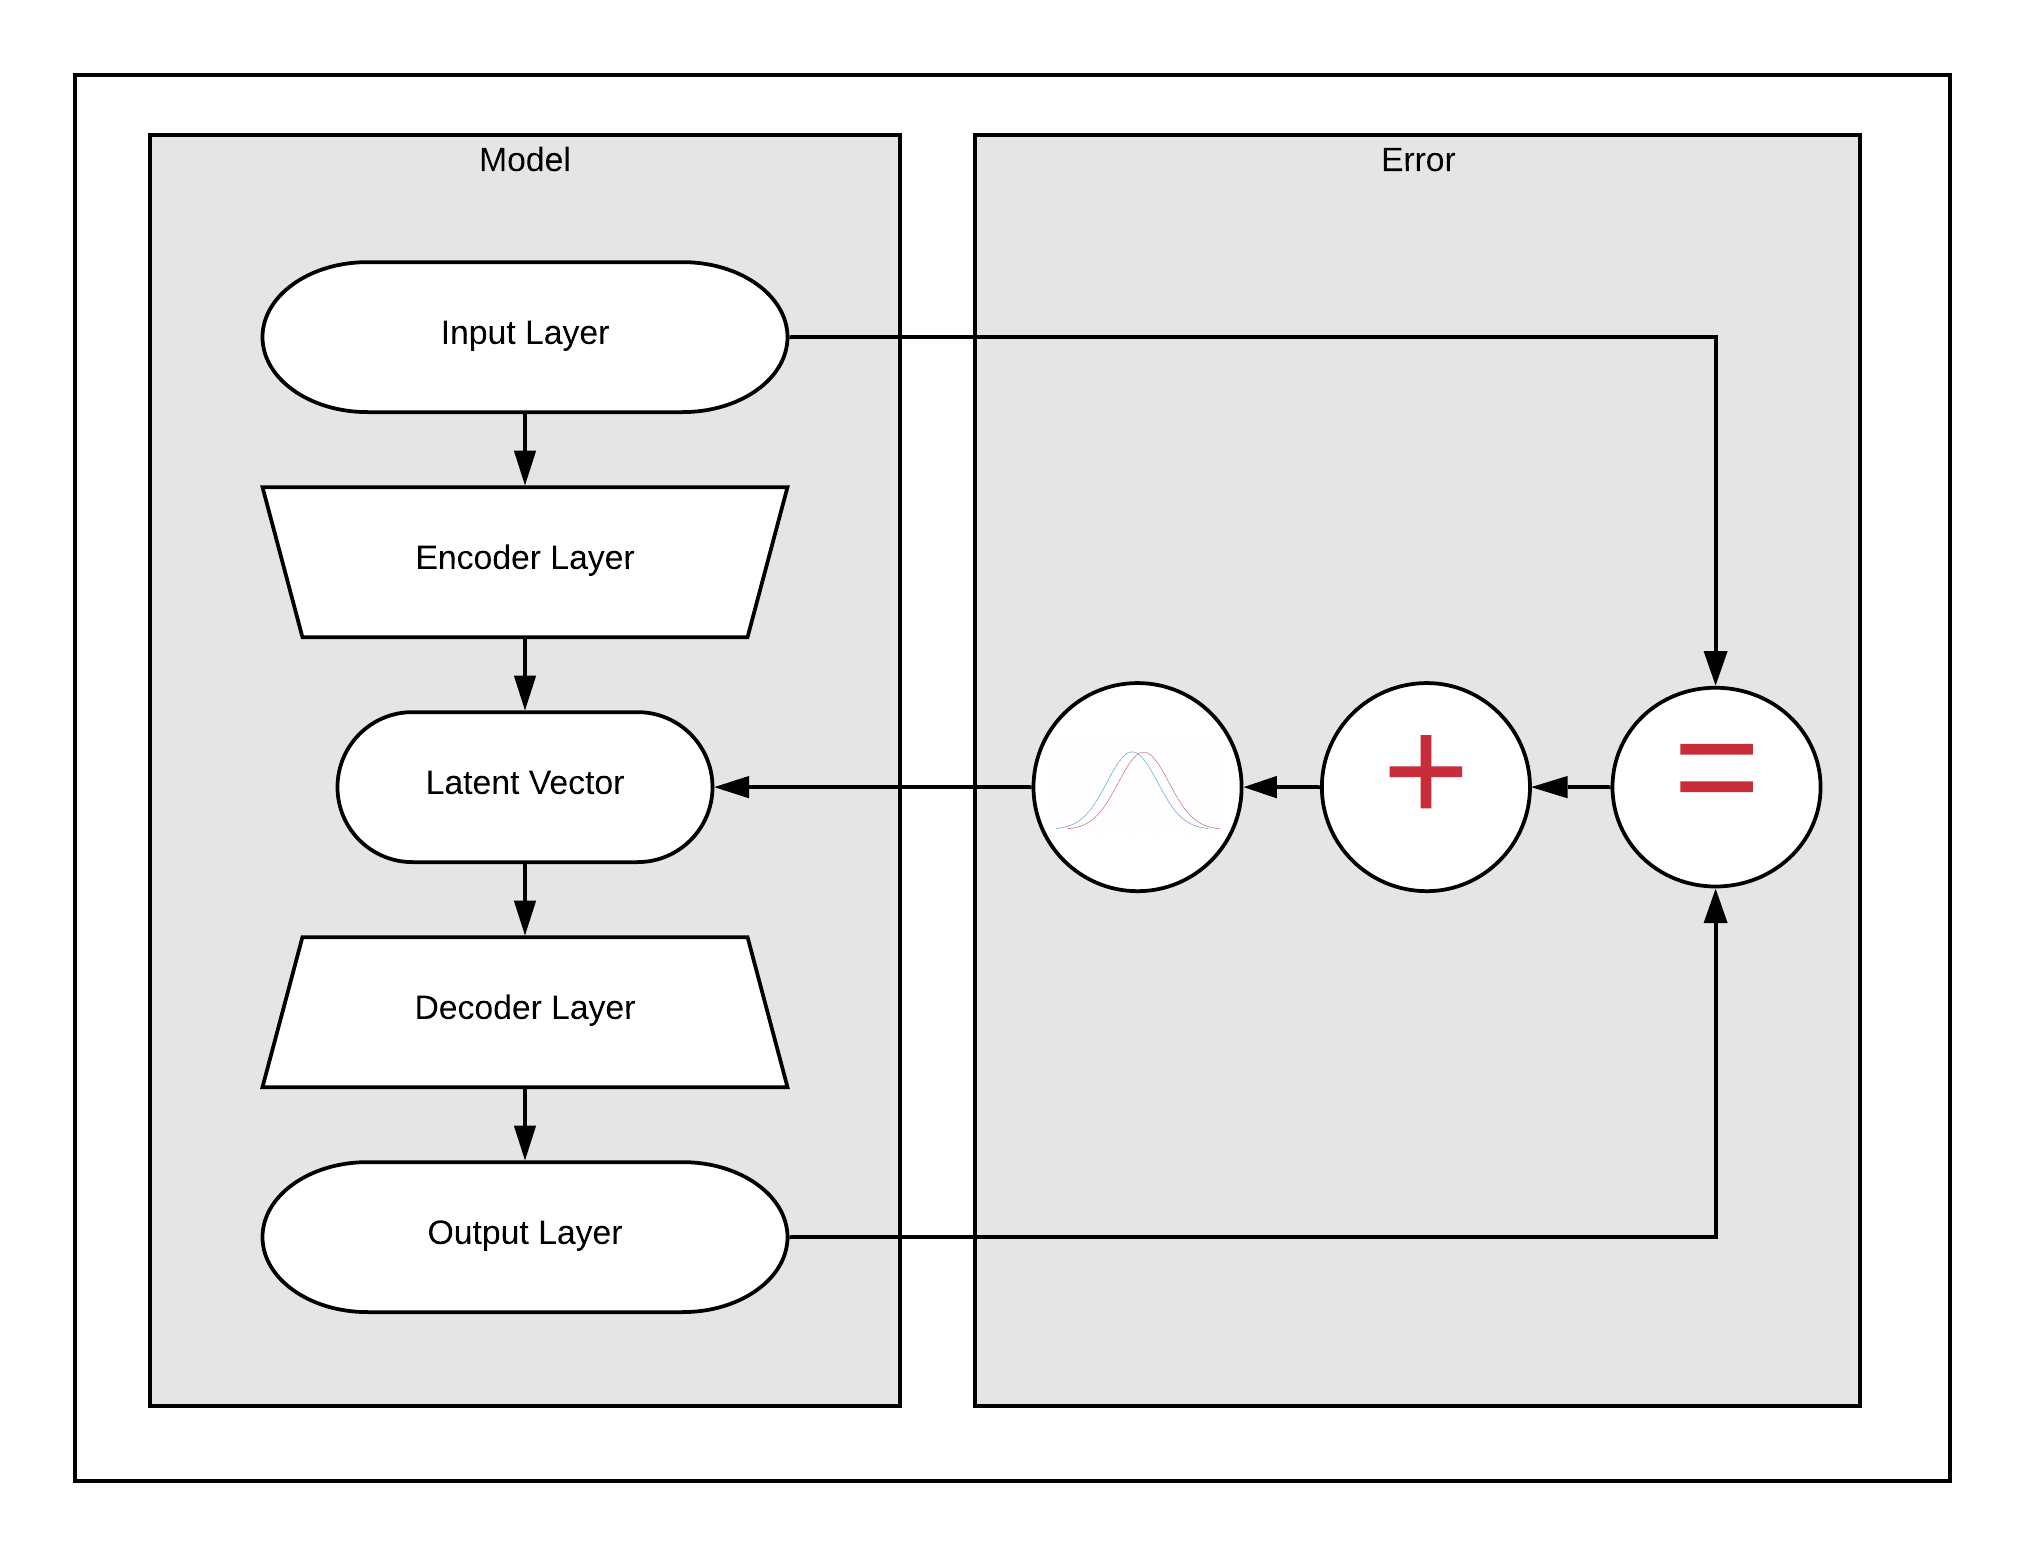
\includegraphics[width=.8\linewidth]{figuras/VAE_Diagram.png}
	\end{center}
	\caption{Flowchart of a variational autoencoder} \label{fig2}
\end{figure}

%\hfill mds
 
%\hfill July 26, 2019

\subsubsection{Encoder layer}

In Bayesian modeling, the distribution of observed variables is governed by latent variables. The latent variables are extracted from a previous density $p(z)$ and related to the observations through the probability $p_\theta(x|z)$. Deep latent gaussian models (DLGMs) are a general class of models where the observed variable is governed by a latent variable hierarchy, and the latent variables at each level of the hierarchy are Gaussian a priory\cite{Rezende2014}.

Normally, in the VAE, a Gaussian distribution is used to sample the latent space.

\begin{equation}
    p(z)=N(0,I) 
    \label{eq1}
\end{equation}


In this way, each local latent variable is related to its corresponding observation through the likelihood $p_\theta(x|z)$, which can be seen as a probabilistic decoder. Using a hidden smaller representation $z$, it decodes it into a distribution over observation $x$.

\subsubsection{Decoder layer}

The decoder is another neural network. Its input is the latent vector $z$, generates the parameters for the probability distribution of the data and has weights and biases $\theta$. The decoder is denoted by $p_\theta (x|z)$. The probability distribution is a multivariate Gaussian.

The loss function of VAE is the negative log-likelihood with a regularizer. Since it is not possible to
generalize the global representation shared by all data points, we can decompose the loss function into terms
that depend only on a single data point $l_i$. The parameters are typically the weights and biases of the
neural networks represented as $\theta$ and $\phi$. The total loss will then be represented by the sum of
all losses $l_i$ for all data points. The loss function $l_i$ for the data point $x_i$ is:

\begin{equation}
    \begin{split}
        l_i(\theta,\phi) = \mathbf{E}_{z~q_\theta}(z ∣| x_i)[log(p_\phi(x_i |∣ z))] \\
        +\mathbf{KL} (q_\theta(z |∣ x_i)∣|| p(z))
        \label{eq2}
    \end{split}
\end{equation}

The first term represent the reconstruction loss, and has the form of a negative log-likelihood of the i-th data point. The expectation is taken with respect to the encoder’s distribution over the representations. This term encourages the decoder to learn how to reconstruct the data. If the decoder’s output does not have similarity with the data, statistically the decoder parameterizes a likelihood distribution that does not place much probability mass on the true data. Poor reconstruction will incur a large cost in this loss function.

The second term is a regularizer. This is the Kullback-Leibler divergence between the encoder’s distribution $q_\theta(z|x)$ and $p(z)$. This divergence measures how much information is lost when using $q$ to
represent $p$, in other words, the divergence of the approximate from the true posterior.

\subsubsection{Inference Network}

An inference network is a flexible construction for parameterizing approximating distributions during inference\cite{Dayan1999}, and it is used on VAE\cite{Rezende2014, Welling} to infer the optimal values of the latent variables given observed data, or to calculate the posterior $p(z∣|x)$. By modeling the true
distribution P(z|X) using simpler distribution that is easy to evaluate, e.g. Gaussian, and minimize the
difference between those two distribution using KL divergence metric, as in \ref{eq2}, which tells us how difference it is $p$ and $q$.

\subsection{sEMG Database}

In this work the "6mov8chFUS" database made available with the BioPatRec platform\cite{Ortiz-Catalan2013} was used. The “6mov8chUFS” database consists of 17 patients, with six individual movement classes selected, such as opening and closing the hand, flexion and extension of the wrist, and prono-supination of the hand, forming 27 possible movements.

The signal was measured as follows: 3 seconds of contraction time with 3 seconds for relaxation between each repetition, repetitions of each movement. 8 bipolar electrodes (disposable Ag / AgCl), 1 cm of electrode diameter, 2 cm of inter-electrode distance for the bipolar. Electrodes were equally spaced around the proximal third of the forearm.

\subsection{Feature extraction}

In order to reduce signal noise, the first step in extracting features was to use a sixth-order bandpass Butterworth filter, 80-450Hz. Additionally, a time window for sampling the signal is selected. In this study, the sampling frequency of the sEMG was 2000 Hz, with a 0.01s window (i.e., ten samples per window).

This stage was subdivided into two steps:

\begin{enumerate}

    \item \textbf{Selection of characteristics:} to extract information from the signal four frequency domain features were used~\cite{Jose2018}:
    \begin{itemize}
    	\item  Spectral Moment;
    	\item  Waveform Length (acumulative changes in the length);
    	\item  Mean;
    	\item  Median;
    \end{itemize}
    \item \textbf{Dimensional reduction:} NCA~\cite{Phinyomark2013} allowed for the dimensional reduction by helping to select the most significant features of the signal. NCA is a supervised learning algorithm for distance metric learning. It learns a linear transformation (of input data) that maximizes, in the transformed space, the average leave-one-out classification performance.
\end{enumerate}

\subsection{VAE Algorithm}
A simple Variational Autoencoder was used for the anomaly detection phase. The encoder stage was compose of three dense layers. The first one have 32 neurons, the second 16 neurons and the third 8 neurons. The sampling inference, which characterizes the variational autoencoder, is made on top of the last layer of the encoder step, which has 8 neurons. All layers in this phase have the Rectified Linear Unit (ReLU) as the activation function.

The decoding stage is the reverse of the encoding. It starts with 8 neurons in the first layer, 16 neurons in the second and 32 neurons in the last. The first two layers have ReLU as the activation function and the third layer, the sigmoid as the activation function.

\begin{figure}[h]
\centering
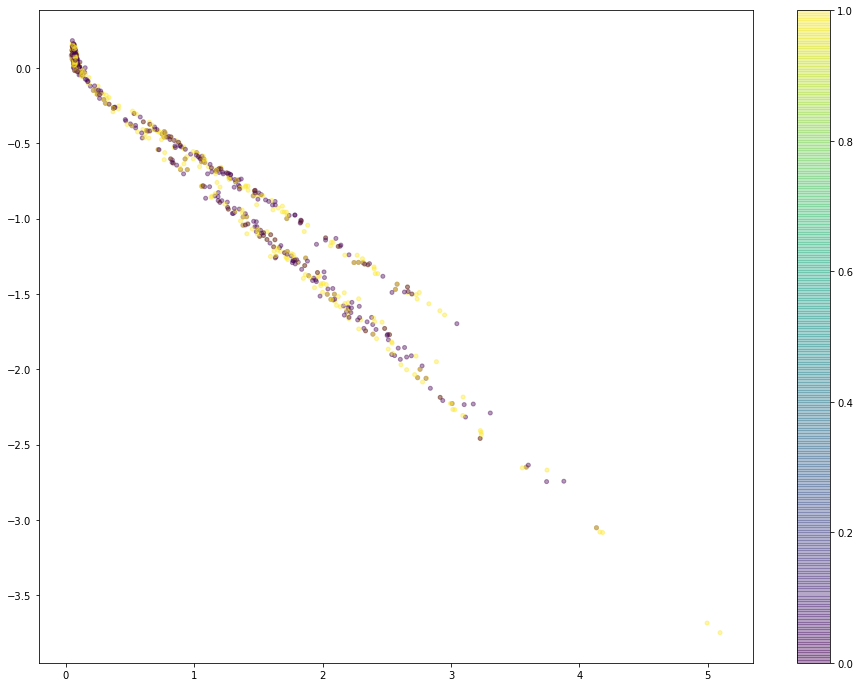
\includegraphics[width=.8\linewidth]{figuras/latent_space_vae.png}
\caption{The latent space representation created by te Variational Autoencoder} \label{fig_lat_space}
\end{figure}

The figure \ref{fig_lat_space} is the dimensionless values of the autoencoder trained with two neurons in the latent layer. The figure represents the representation of the anomalies found when the patient starts to move. With that output of the latent space, a simple perceptron network is used to detect whether the patient is moving or resting.

\section{Results}

In this experiment, a 0.01s window (10 samples) was used. With this window size, normal classification methods cannot accurately classify the movements classes or even differentiate the resting state of movement. Through the use of auto-encoder as an anomaly detector, it was possible to determine the moment when the movement really started.

The figure \ref{fig_lat_space_rep} is the representation of the difference between the rest movement state in the latent space of the variational autoencoder. For the construction of the image the latent space was dimensioned with 4096 neurons. The output of the neurons has been scaled to a 64 by 64 square shape and the image was made.

\begin{figure}[h]
    \begin{center}
	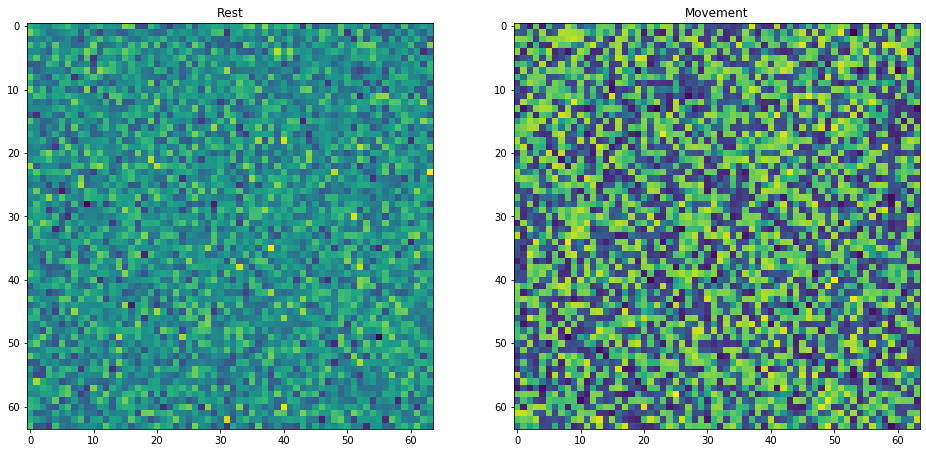
\includegraphics[width=.8\linewidth]{figuras/latent_space_as_image.png}
	\end{center}
	\caption{A expanded latent space, to represent the diference between the rest and the rest and the movement state. In this image the latent space was dimensioned to be 64 x 64 to facilitate the diference visualization.} \label{fig_lat_space_rep}
\end{figure}

It is worth remembering that, although the detection of the anomaly only needed eight neurons to be able to perform successfully, the representation of the latent space needed to be enlarged so that the difference was visible to our eyes.


\section{Conclusion}

The results obtained demonstrate the feasibility of the variational autoenconder as an anomaly detector for the sEMG signal. Furthermore, by separating the resting state from the other classes of movement, the entropy of the system is reduced, facilitating the future classification of the other classes of movement.

By using VAE, which is specialized in separating classes in their latent space, movement detection has been simplified and its computational cost has been greatly reduced. Although the training was done only using the offline signal, simulating the acquisition of the signal online proved to be extremely efficient.

In this study, the auto encoder was used only as an anomaly detection instrument, but its use is not limited to that. As shown in figure ~\ref{fig_lat_space_rep}, the autoencoder can be used to increase the separation between classes just by increasing the size of the latent space. This technique can be used in further studies to improve the system accuracy.

\section{Conflict of Interest}
The authors declare that they have no conflict of interest.


\bibliography{referencias}

\end{document}
